\Chapter{A különböző rácsok a játékokban}

\section{Rácsok összehasonlítása}

Legyen szó társasjátékról vagy számítógépes játékról, az egyik leggyakrabban használt rács a négyzetrács. Egyszerű, könnyen kezelhető és jól illeszthető a számítógép kijelzőjére.
\newline A cellák pozícióit a \textit{Descartes-féle derékszögű koordináta-rendszer} ($x, y$) segítségével határozhatjuk meg. 
\newline Kirajzolásához ismernünk kell a cella méreteit (szélesség, magasság) illetve a rács méreteit (oszlopok, sorok száma). 
\newline A nyilvántartáshoz ismernünk kell a viszonyítási pontot (origó), illetve tudnunk kell az objektum pozícióját ($x, y$).
\newline
\newline Könnyen kezelhetősége mellett viszont van egy nagy hátránya.
Egy négyzetnek nyolc szomszédja van. Oldalain keresztül vízszintesen, valamint függőlegesen 2-2 szomszédja érhető el. További négy szomszédja átlósan található meg. A problémára akkor figyelünk fel, amikor megvizsgáljuk a távolságot a különböző szomszédok között. A vizsgálathoz tegyük fel, hogy az oldalak hossza 1. Ha a négyzetek középpontjához viszonyítunk, akkor a függőlegesen és a vízszintesen lévő szomszédok távolsága 1, míg az átlósan lévők távolsága $\sqrt{2}$. Ez azért baj, mert így az átlós szomszédok torzítják a távolságot, ezáltal nem lesz arányos a mozgás minden irányban.

\begin{figure}[h!]
\centering
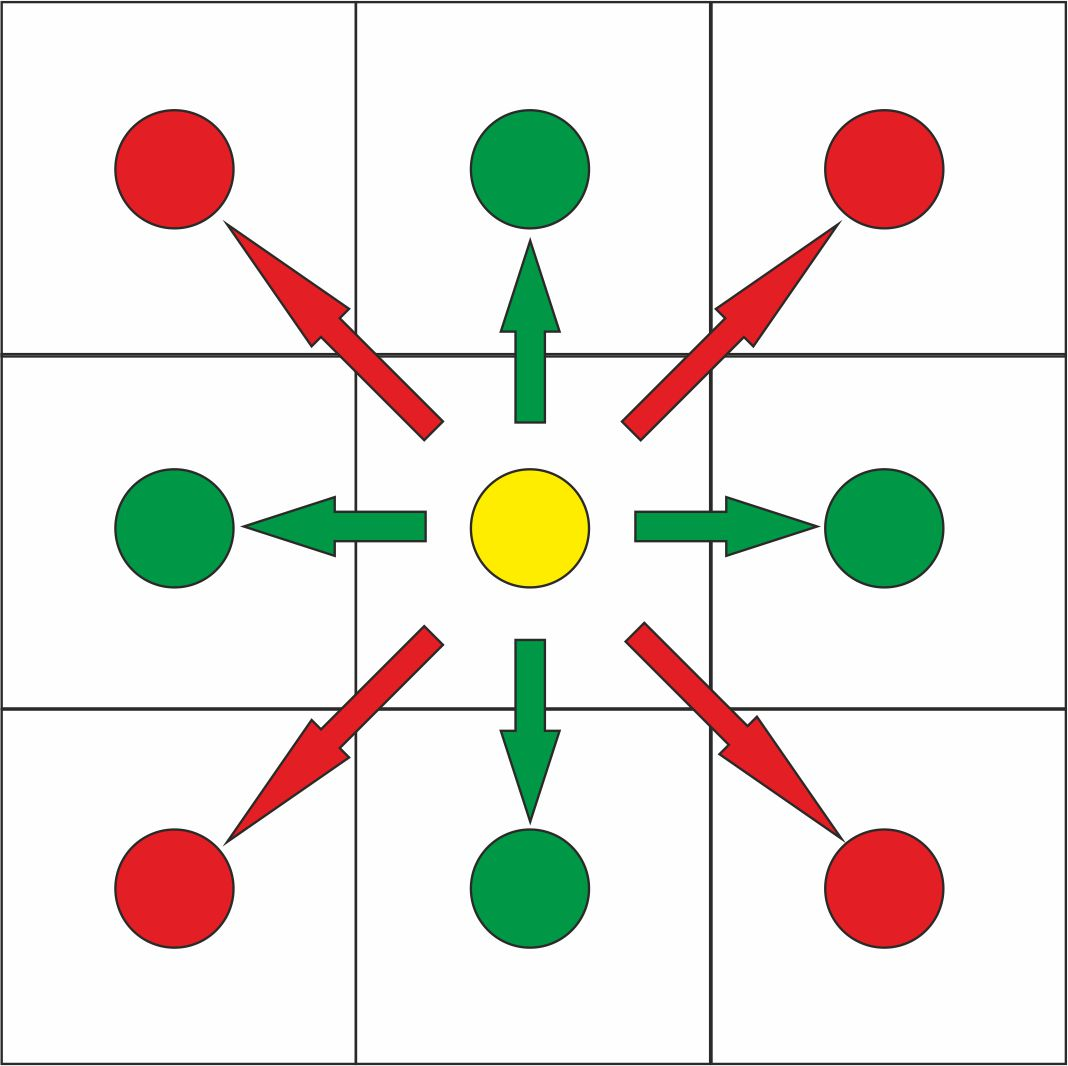
\includegraphics[scale=0.4]{kepek/SqDistance.jpg}
\caption{A szomszédok távolsága a négyzetrács esetén}
\label{fig:SqDistance}
\end{figure}

\noindent A két fajta szomszéd közötti különbség miatt vetődnek fel bizonyos kérdések: Hogyan kezeljük az átlós mozgást? Egyáltalán engedélyezzük-e az átlós mozgást? A mozgás természetessége és arányossága érdekében hogyan érhetnénk el azt, hogy minden szomszéd azonos távolságra legyen egymástól?
\newline
\newline A problémára több megoldás is létezik:

\begin{itemize}
\item Nem alkalmazunk átlós mozgást. Ez a legegyszerűbb megoldás, amit az egyszerűsége miatt gyakran használunk.
\item Egy kevésbé elterjedt megoldás, hogy maradunk a négyzeteknél, viszont minden második sort/oszlopot eltolunk az oldal hosszának a felével. Ekkor az összes szomszéd hasonló távolságra kerül.

\begin{figure}[h!]
\centering
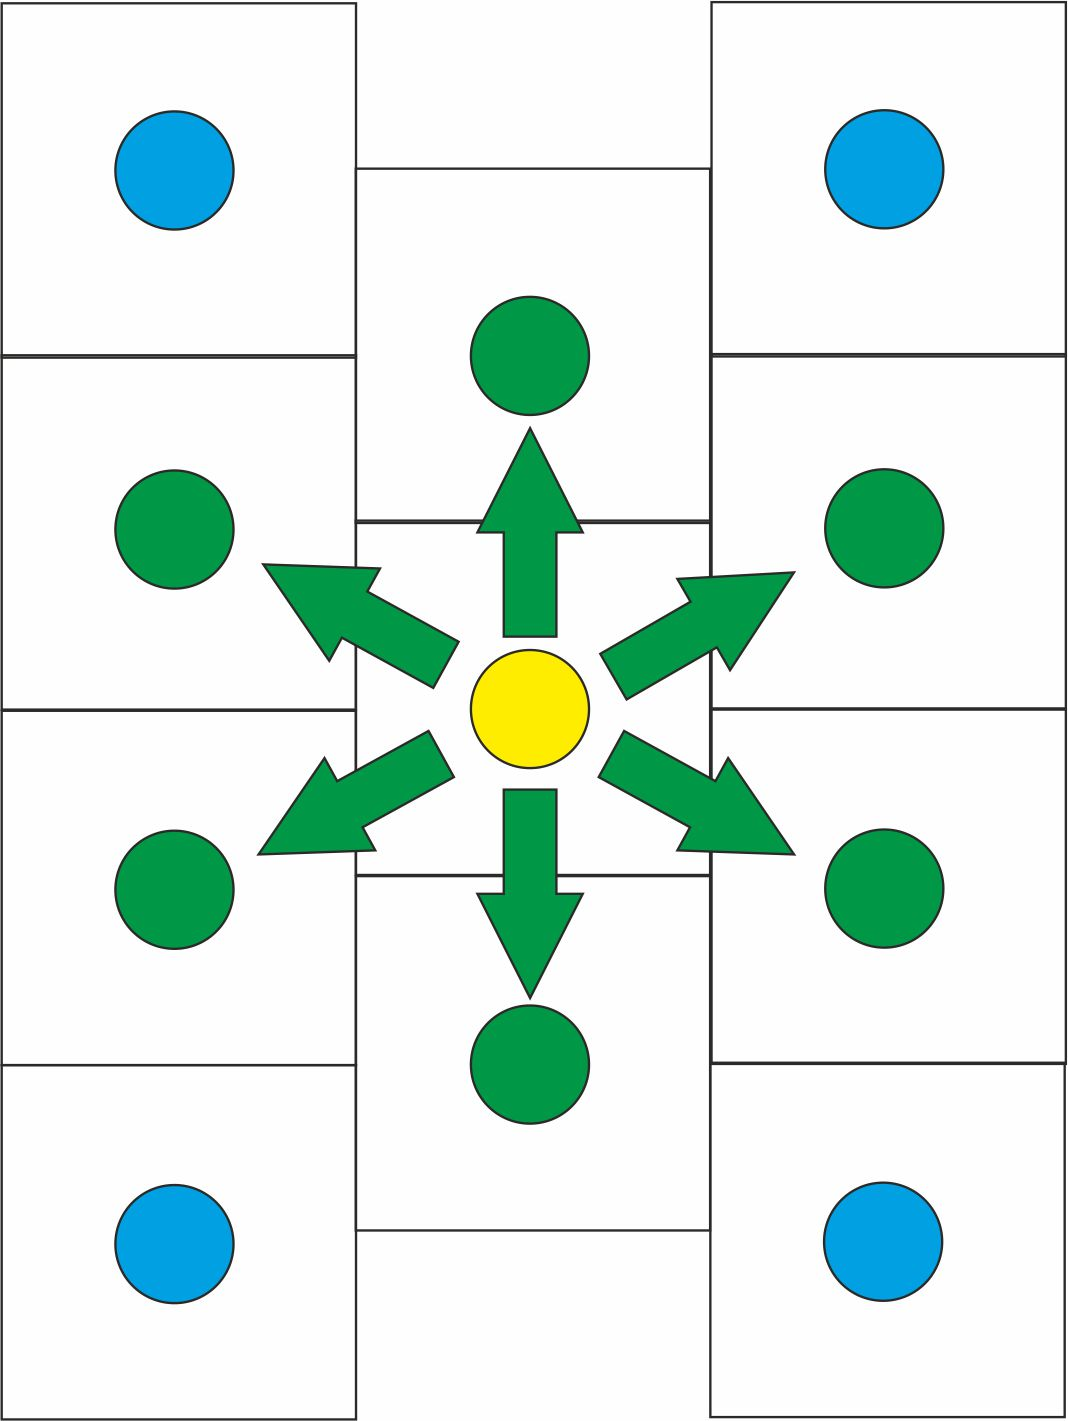
\includegraphics[scale=0.3]{kepek/SqOffsetDistance.jpg}
\caption{Az eltolásos négyzetrács esetén a távolságok}
\label{fig:SqOffsetDistance}
\end{figure}

\item A leggyakoribb megoldás a hexagonok használata a négyzetek helyett. A négyzethez hasonlítva a hatszögnek csak hat szomszédja van (nyolc helyett). Ezek közül mindegyik oldal szomszéd, és nincs olyan szomszédja ami a sarkokhoz esne. Ezáltal minden szomszéd egyenlően 1 távolságra van.
\end{itemize}

\noindent A hexagonrácsot azért szokták játékokban használni mert kevésbé torzítják a távolságokat mint a négyzetrács. Ez azért van mert nincs átlós szomszédja ellentétben a négyzettel.

\begin{figure}[h!]
\centering
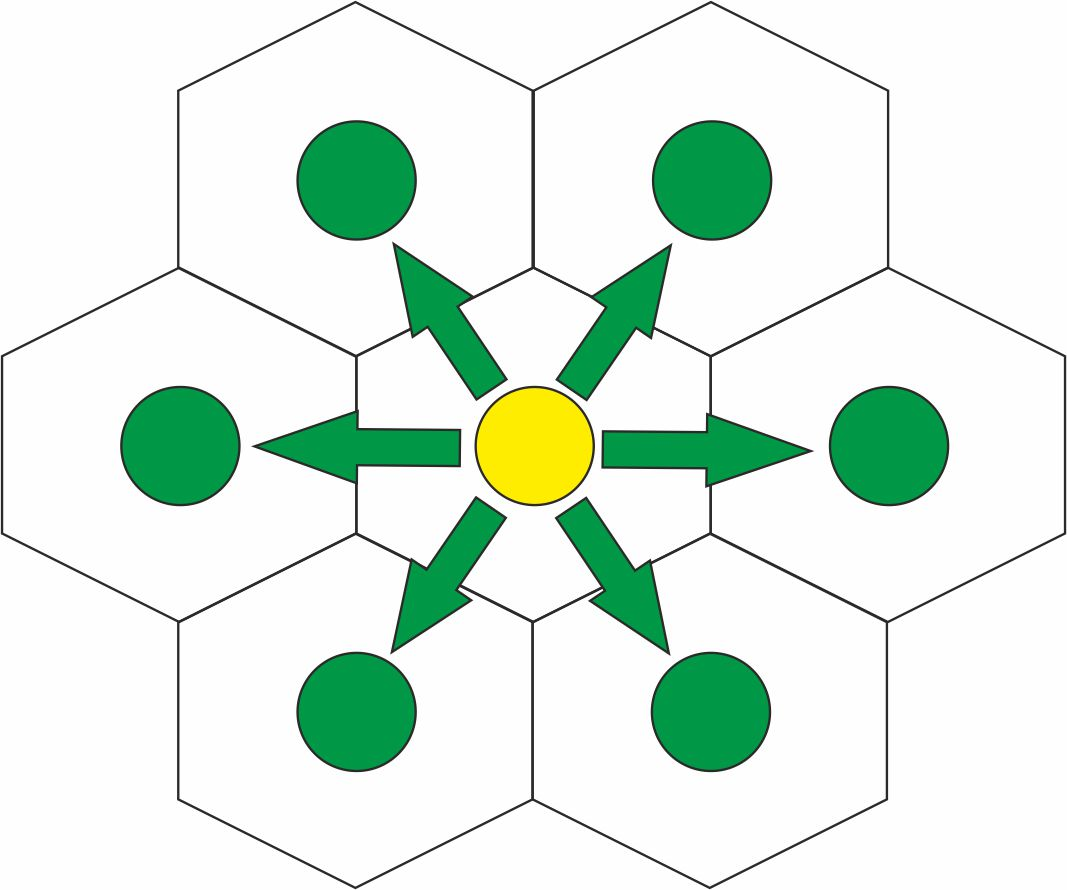
\includegraphics[scale=0.4]{kepek/HexDistance.jpg}
\caption{A szomszédok távolsága a hexagonháló esetén}
\label{fig:HexDistance}
\end{figure}

\noindent A fő indok a hexagonháló mellett az eltolt négyzethálóval szemben az, hogy sokkal kézenfekvőbb a hat lehetséges mozgási iránynak a használata. Sok ember számára zavaró vagy nem teljesen egyértelmű első ránézésre, hogy hogyan történik a horizontális mozgás az eltolt négyzetrács esetén. Emellett még esztétikailag is kellemesebb érzetet nyújt a felhasználó számára.

\section{Rácsok felhasználása}

Alapvetően mindkét rácsnak megvan a maga helye a játékfejlesztésben. 
\newline
\newline Mivel a beltéri helyszínek (szobák) és az azon belüli elemek (bútorok) általában téglalap alakúak, praktikusabb a négyzetrács használata. A négyzetrács a falakhoz tökéletesen illeszkedik, ugyanakkor a hexagonok esetében problémák merülnek fel. Ugyanis a hexagonok nem fognak szabályosan illeszkedni a falak mentén. Erre kétfajta megoldás létezik: a fal menti hexagonokat elvághatjuk, vagy másik megoldás, ha nem töltjük ki a fennmaradó helyeket.

\begin{figure}[h!]
\centering
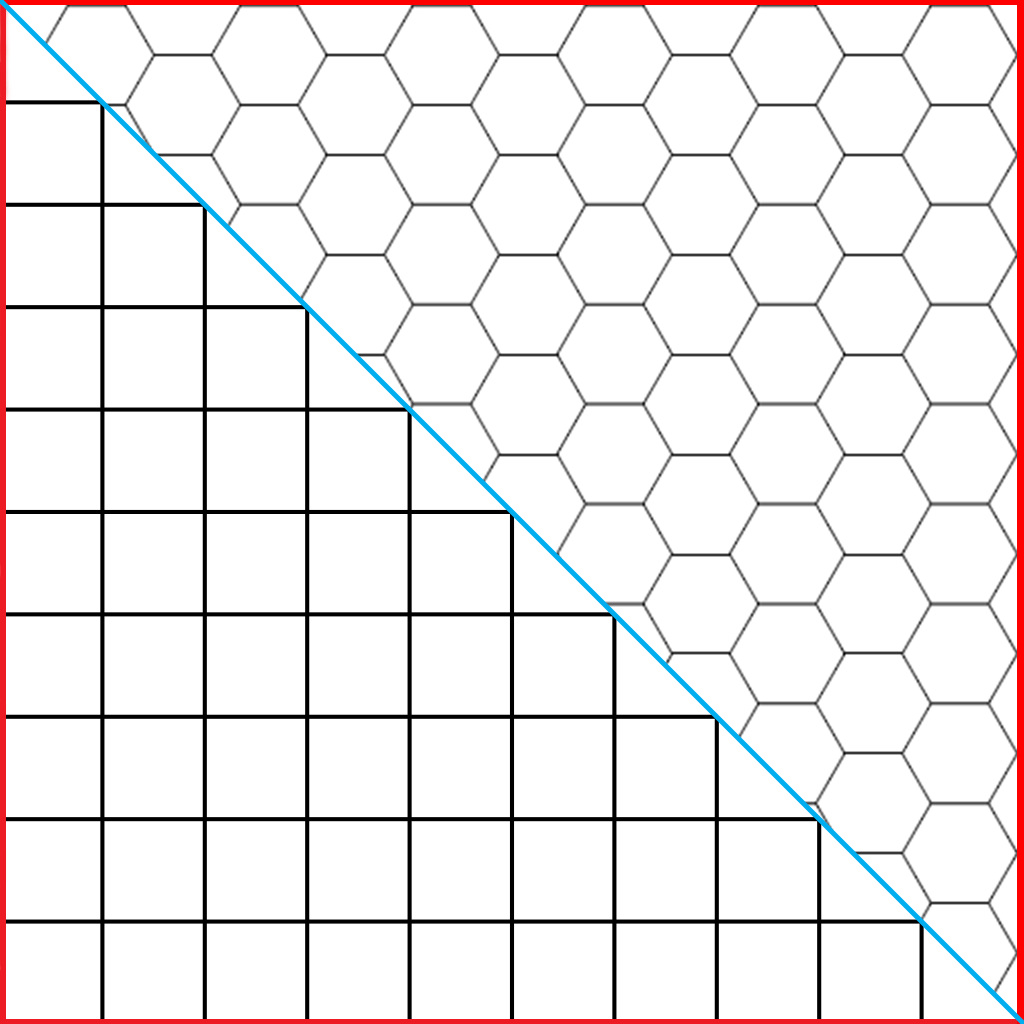
\includegraphics[scale=0.1]{kepek/SqVsHex.png}
\caption{A hexagon és a négyzet rács zárt térbeli összehasonlítása}
\label{fig:SqVsHex}
\end{figure}

\noindent Egyik megoldással sem lehetünk maradéktalanul elégedettek, ha elvágjuk a hexagonokat: 

\begin{itemize}
\item Ha csak kihagyjuk a széleken a hexagonokat amik nem férnek el az a felhasználó számára furcsa összhatást nyújthat.
\item Ha mindenképpen hexagonokat  szeretnénk használni kis méretű térképen (pl: $8 \times 20$), akkor lehetőleg ne egy zárt szobában alkalmazzuk hanem szabad téren (pl: mező, erdő, tengerpart) vagy próbáljuk a hexagon rács széleihez igazítani a környezetet.
\item Kültéren, falak hiányában ezek a problémák nem merülnek fel. Emiatt, valamint a négyzetrács átlós mozgásával kapcsolatos problémák miatt előnyösebb a hexagonháló használata ezekben az esetekben.
\end{itemize}

\section{Rácsok részei}

A rácsoknak három különböző része van: a lapok, az élek és a csúcsok. Minden lap két dimenziós felület élek által határolva. Minden él egy dimenziós szakasz aminek mind a két végén csúcsok találhatóak. Minden csúcs nulla dimenziós pont. 

\begin{figure}[h!]
\centering
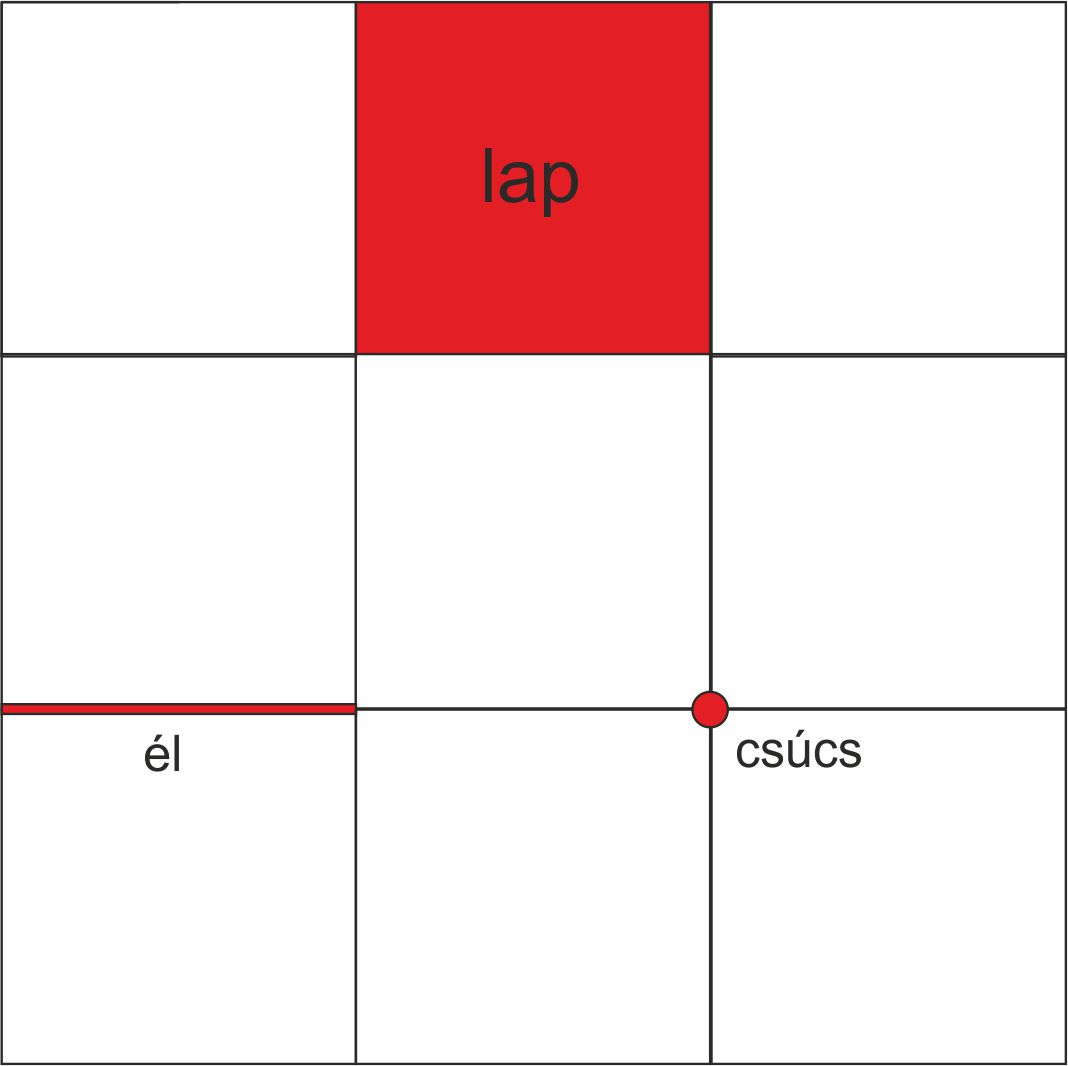
\includegraphics[scale=0.4]{kepek/PartsOfGrid.jpg}
\caption{A rács részei}
\label{fig:PartsOfGrid}
\end{figure}

\noindent A játékok nagy többségében közös az, hogy a rácsoknak csak az egyik részére koncentrálnak. A nyugati játékoknál mint a sakk vagy a dáma a rácsnak a lap részén van a fókusz ellentétben a keleti játékokkal mint a Go vagy a Csillaghalma (Chinese Checkers), ahol a csúcsokon van.
\newline
\newline Lapok, élek és csúcsok feltűnnek a különböző poligonokból álló  térképek esetén is. Egy olyan algoritmus ami a lapok, élek vagy csúcsok alapján működik de nincs szükség koordinátákra az működni fog ilyen térképek esetén is.

\begin{figure}[h!]
\centering
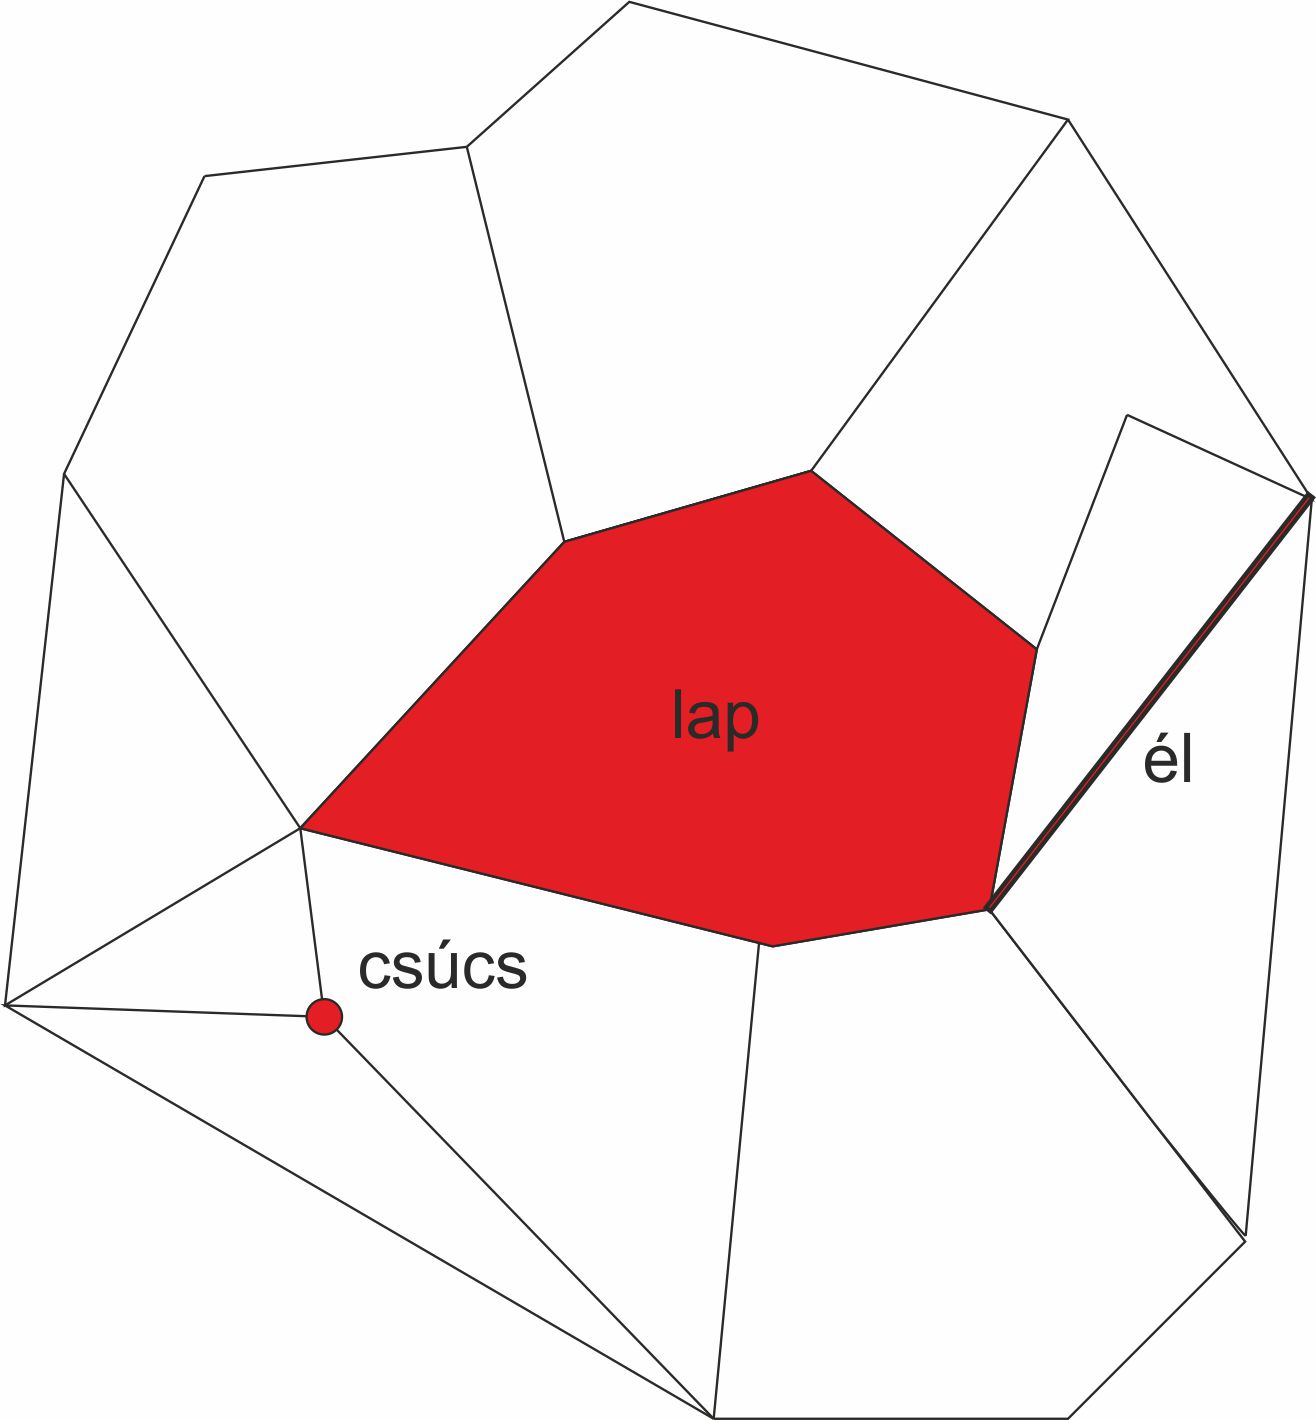
\includegraphics[scale=0.4]{kepek/PartsOfGrid2.jpg}
\caption{Különböző poligonokból álló térképen a rács részei}
\label{fig:PartsOfGrid2}
\end{figure}

\noindent A gráf struktúra megengedi számunkra, hogy gráf algoritmusokat (például: \textit{legrövidebb út}) használjunk a térképen. A rácsok és a poligonális térképek átalakíthatóak gráf struktúrákra azáltal, hogy minden lapból csomópontot és minden lapok közötti élből pedig a csomópontok közötti gráf éleket készítünk.

\section*{Használatuk játékokban}

A számítógépes játékok mind a három típust használhatják, de a lap a leggyakoribb. Épületek, terület típusok (fű, sivatag, stb.) és a terület birtoklás a lapokat használja. Az “áramlás” (“flow”) algoritmusok (ami szimulálja az áramlását a víznek, embereknek, termékeknek, stb. a szomszédos csempék között) használják az éleket. Az élek a két lap közötti kapcsolatot írják le, tehát megadják, hogy az egyik lapról elérhető a másik lap. A magasság a csúcsokat használja. Az utakhoz lehet használni a lapokat és az éleket is.

\section{Ábrázolás}

\subsection{Négyzet}

A négyzetháló esetén van a legkönnyebb dolgunk ismételten. A négyzetek alapvetően egy féle képpen állnak, úgy, hogy a lapjuk áll felfelé.  A négyzeteket ebben az esetben, úgy tudjuk egymás mellé helyezni, hogy a szomszédos négyzetek középpontjai közötti távolság megegyezik az oldal hosszal. 
\newline
\newline Abban az esetben sincs sokkal nehezebb dolgunk, ha úgy döntünk, hogy az eltolt négyzetrácsos megoldást választjuk, ebben az esetben minden páros/páratlan sort/oszlopot kell eltolnunk az oldalhosszának felével.

\subsection{Hexagon}

A hexagonok alapvetően kétféleképpen állhatnak. Az egyik lehetőség, hogy az egyik csúcs van felül, a másik lehetőség, hogy az egyik oldal van felül. 
\newline
\newline A következő lépésként vizsgáljuk meg, hogy hogyan tudjuk egymás mellé elhelyezni a hexagonokat.
\newline
\newline A \textit{felül hegyes} elrendezés esetén vízszintesen a hexagon szélességével, függőlegesen pedig a hexagon magasságának a $\frac{3}{4}$ vel kell eltolni következő hexagont. Ezen kívül minden páros/páratlan sort vízszintesen a szélesség felével kell még eltolni.
\newline
\newline A \textit{felül lapos} elrendezés esetén vízszintesen az egymás melletti hexagonok közötti távolság a hexagon szélességének $\frac{3}{4}$ része. Függőlegesen minden páros/páratlan oszlopot a magasság felével kell eltolni.

\begin{figure}[h!]
\centering
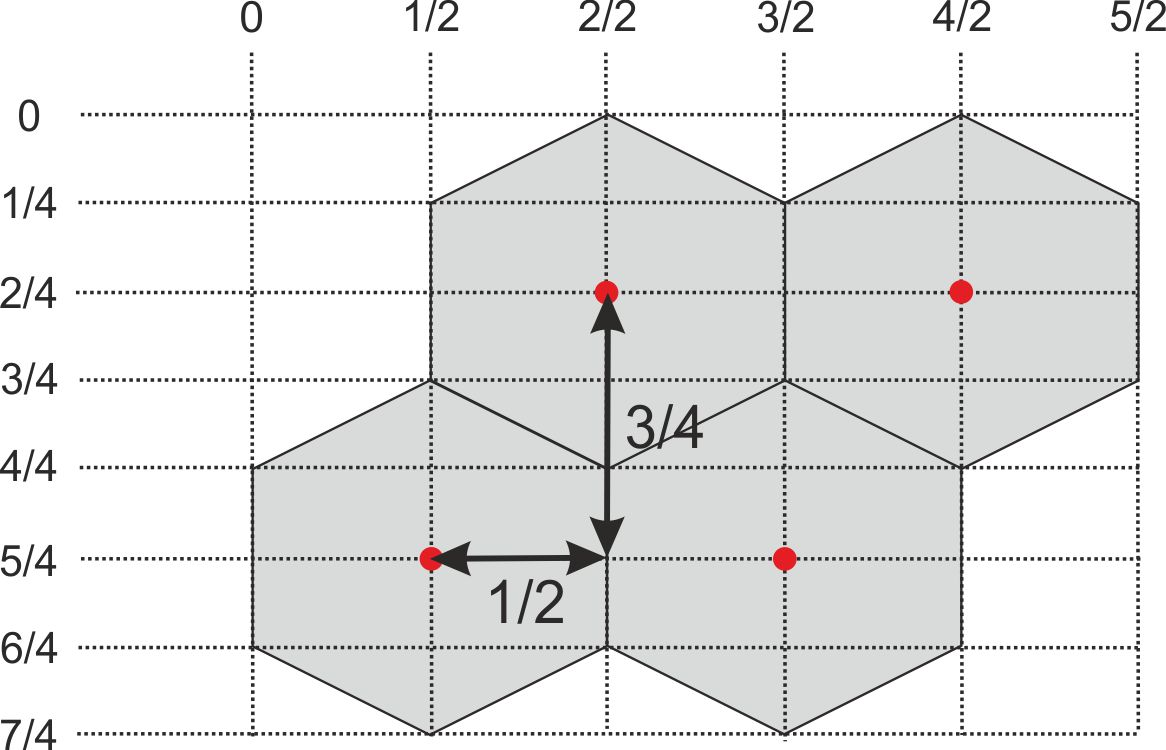
\includegraphics[scale=1.0]{kepek/PointyTop.jpg}
\caption{\textit{Felül hegyes} elrendezés esetén az eltolások}
\label{fig:PointyTop}
\end{figure}

\begin{figure}[h!]
\centering
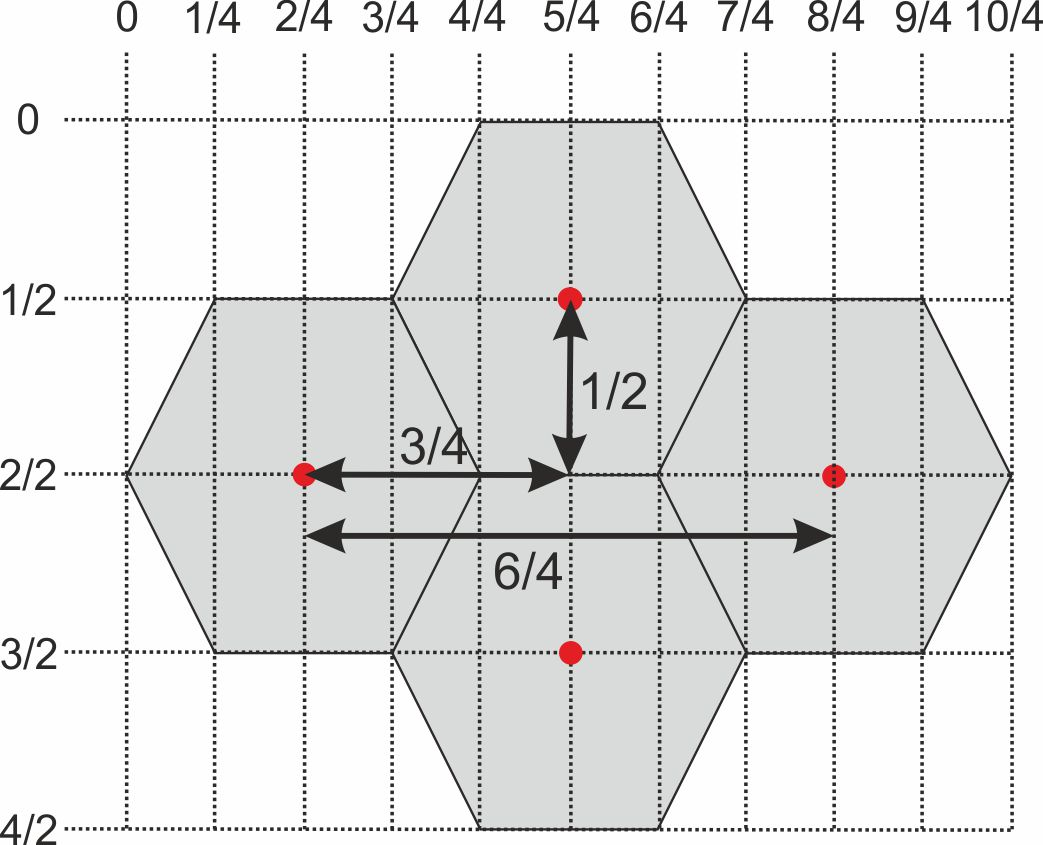
\includegraphics[scale=1.0]{kepek/FlatTop.jpg}
\caption{\textit{Felül lapos} elrendezés esetén az eltolások}
\label{fig:FlatTop}
\end{figure}
